%\documentclass{acmsiggraph}
%\documentclass{acm_proc_article-sp}
\chapter{Analytical Model}
\def\tracea{UDP-High_result}
\def\traceb{UDP-Low_result}
\def\tracec{DCCP_result}
\def\mesha{Happy}
\def\meshb{Horse}
\def\meshc{Thai}
\def\mesh_h{Happy2}

\section{Introduction}
\label{s:model:intro}
    Advances in 3D scanning technology and mesh reconstruction
    algorithms have lowered the barrier in creating complex mesh
    objects and sharing them over the network.  For instance,
    software such as
    ZBrush is enabling easy creation of complex digital sculpture.
    The Stanford's Digital Michelangelo Project
    \cite{levoy00digital} digitized statues made by Michelangelo
    and provided a software, ScanView \cite{koller04protected},
    to allow users to remotely view the 3D version of the statues.
    Similar projects include the Digital Sculpture Project \cite{deroos2004dsp}
    and the project to digitize Rodin's sculptures \cite{miyazaki2006dab}. 
    Second Life, an online virtual world, is driven mostly by 
    user-created 3D objects, which are downloaded 
    on demand as users explore the virtual world.  
    These signs suggest that an increasing amount of
    3D mesh data will be available for remote viewing over
    the Internet.

    This paper targets at networked applications that require 3D meshes with high quality,
    such as virtual museum and virtual earth
    The amount of data constituting a high quality 3D mesh can be
    huge. For example, the statue of David, from the Digital
    Michelangelo Project, consists of 2 billion polygons.  After
    lossless compression, the total data size is 32 GB.  To reduce
    waiting time when downloading such a huge amount of data, a common
    technique for remote viewing is to encode a 3D mesh
    progressively \cite{lod}, allowing a low resolution version
    of the mesh to be transmitted and rendered with lower latency.
    The refinement information is continuously being transmitted,
    and the quality of the rendered model is incrementally improved
    over time.  Such progressive rendering is also useful in the
    case of virtual worlds such as Second Life. 
    In such applications, even though the models are typically smaller and simpler, 
    an arbitrary scene can contain numerous objects.
    Furthermore, such applications are interactive in nature.
    It is thus desirable for users to quickly visualize a coarse version
    of the scene first, instead of waiting for full objects to be
    downloaded before they can be displayed.
    %Note that our target applications are not 3D games, where strict high
    %interactivity is required and high quality 3D meshes are not commonly used.

    Progressive coding of meshes, much like progressive coding of
    video, introduces dependencies between data.
    Dependencies between data units can cause delay in decoding
    when sent over a lossy network -- a data unit
    cannot be decoded and displayed if one of the other data units
    it depends on is not received correctly. For example, in the
    context of video streaming, MPEG-encoded frames are inter-dependent:
        an I-frame has to be received and decoded properly
    before being able to decode the subsequent P-frames and B-frames
        referencing this I-frame (either directly or indirectly).  Another
    example is in layered coded video, where the base layer has
    to be received before the enhancement layers can be decoded.
    The effects of dependencies in the context of video streaming
    have been well studied in the literature \cite{boyce98}.   Multi-resolution 3D
    objects also have dependencies between different level of details.
        For progressive meshes, the mesh is refined by successive
    \textit{vertex splits} (see Figure~\ref{model:split}).  Thus,
    dependencies exist between the original vertex and its one
    ring (the direct neighbors of the vertex)
    and the vertices and triangles created by the vertex split.
    The effects of these dependencies on decoded mesh quality, however,
    are not well understood.  Due to the fundamentally different
    nature of progressive mesh and video data, what we learn from
    video streaming research does not apply.  This paper aims to study
    the effect of dependencies in progressive mesh streaming by
    proposing an analytical model, relating the decoded mesh quality
    of progressive mesh to packet loss rate, given the dependencies
    among vertex splits.

    The decoded mesh quality at a given time $t$ is determined by 
    the vertex splits that are decoded before $t$ and their contribution to the overall mesh quality.
    To estimate the decoded mesh quality at time $t$, our analytical model
    predicts the decoding time of each vertex split.  The total contribution of vertex
    splits decodable before $t$ gives the quality.  To predict the decoding time, we first
    express the expected time for receiving each packet
        in terms of loss rate, round trip time, and sending rate.
    A received vertex split has to wait for the vertex splits
    it depends on to arrive before it can be decoded.
    Therefore the received time of a vertex split is not always equal to its decoding
    time.  Our model gives an expression for the expected
    decoding time given the dependencies among the vertex splits.
    Furthermore, we propose
    a metric to measure the contribution of 
    vertex splits to the
    decoded mesh quality. The decoded mesh quality then can be computed 
    after we know the expected decoding time of every vertex split
    and its contribution.

    Our analytical model is useful in several ways.  First,
    we can analytically evaluate different strategies for streaming
    a progressive mesh.  For instance, packetization of vertex
    splits affects the intermediate decoded mesh quality
    at the receiver.  Evaluating different packetization scheme
    using simulation is an option, but
    it may take many experiments to obtain accurate
    expected values.  Our model computes the expected value easily.
    Second, our model can also help in developing a better sending
    strategy.  The quality of the decoded mesh depends on
    various factors, which include not only network conditions such
    as loss rate and round trip time, but also the order, the
    dependency, and the importance of the data.
    The last three factors are in turn affected by the packetization
    strategy.  Our model can estimate the effect of each factor on the
    decoded mesh quality.
    As such, we can make the right trade-off between these factors
    during transmission to improve the quality.
    Finally, we derive closed-form expressions in two extreme cases,
    giving us insights into the importance of dependencies on the
    decoded mesh quality.

    %Now we clarify the scope of this paper.
    %First, although some other representations
    %of 3D objects exist, such as pointed based representations, we concentrate on 3D meshes. 
    %We are not saying 
    %mesh is the only or the best representation, but it is the most popular one.
    %Moreover, progressive mesh supports finer granularity of progressivity compared with progressive pointed based methods.
    %Nonetheless, our model actually can be applied to any partially ordered data. 
    %For example, we successfully applied it on streaming of digitized plants \cite{plant:seb}
    %Second, in our implementation, only manifold meshes are supported. Most Statues could be represented 
    %as manifold-meshes, and every non-manifold meshes could be transformed to manifold meshes.
    %Third, we only consider static meshes in this paper, and to support the animation is an interesting 
    %future research topic.  
    %(Geraldine)Let us now clarify the scope of our paper. 
    %First, the analysis and strategy we proposed to apply to any partially ordered data 
%    (Multi-resolution 3D models are indeed partially ordered chunks), 
%    e.g. pointed based model organized as QSplat tree. 
%    Here we concentrate on progressive 3D meshes. 
%    Meshes are not necessarily the best representation, 
%    but they are the most popular one. 
%    Moreover, progressive mesh supports finer granularity of progressivity 
%    than other multi-resolution representations. 
%    Nonetheless, our model has actually being applied to other partially ordered data, 
%    digitized plants \cite{plant:seb}.

    Our analytical model is general and can be applied to any 
    partially-ordered data without playback deadline.  We
    choose to concentrate on progressive 3D meshes (which are indeed 
    partially ordered chunks) in this paper. 
    While meshes are not necessarily the best 3D representations, they 
    are popular and support finer granularity of progressivity 
    than other multi-resolution representations. 
    Other examples of such partially-ordered data include point-based models 
    organized as QSplat trees \cite{rusinkiewicz:qsplat} and digitized plants.  
    We have actually applied our analytical model to the latter \cite{plant:seb}.
    
    A preliminary version of this analytical model was previously published 
    \cite{cheng07analytical}.  In this journal version, we extended our work
    with detailed proofs and analysis, as well as extensive validation of our 
    model under a variety of network conditions using different progressive mesh models.

    The rest of the paper consists of six sections. Section~\ref{s:model:bg} provides the background on this paper.
    We describe progressive mesh and how it
    introduces dependencies (Section~\ref{s:model:mesh})
    and present related work in the area
    of 3D objects streaming (Section~\ref{s:model:related}).
    %Section~\ref{s:metric} introduces our evaluation metric
    %for intermediate decoded mesh quality.
    Section~\ref{s:model:model} introduces our analytical model.
    We then describe the applications of our model.
    In Section~\ref{s:model:effect}, we study two hypothetical extreme
    cases, and show the effect of dependencies on
    decoded mesh quality.
    In Section~\ref{s:model:quality}, we show how our
    model can be used to analytically compute the expected
    decoded mesh quality and how this expected quality
    %Section~\ref{s:expected_quality}
    %shows how our model can be used in computing the expected
    %rendering quality given the dependencies and packet loss
    %probability.
    can be used to design a packetization strategy for transmitting
    progressive mesh.  Section~\ref{s:model:experiment} presents validation
    of our model and evaluation of the proposed packetization strategy,
    using network traces using UDP and DCCP under various
    network conditions.  
    Section~\ref{s:model:conclude} concludes by
    reflecting on the insights we gain from our model and its
    implications.

\section{Background and Related Work}
\label{s:model:bg}
\subsection{Progressive Mesh}
\label{s:model:mesh}

    Progressive transmission and rendering of 3D objects
    requires multi-resolution representations of data. One such 
    representation, progressive mesh, is proposed by Hoppe
    \cite{hoppe96progressive}.
    The technique is based on an
    operation called \textit{edge collapse}, and its reverse
    operation, \textit{vertex split}.  Given a (non-progressive)
    3D mesh, the technique applies a series of edge collapses,
    simplifying the model by reducing the number of vertices and
    faces.  The final, simplified model obtained after this
    process becomes the \textit{base model}.  Given a base model,
    we can reconstruct the original model by reversing
    the edge collapse operations through \textit{vertex splits},
    incrementally adding new vertices and faces. So, a
    progressive mesh can be represented by the base
    model and a series of vertex splits.  There are
    dependencies between vertex splits and the base model, as well as
    among the vertex splits.  A vertex split
    operation might need a vertex or a face created by another
    vertex split as input.  Figure~\ref{model:split} illustrates edge
    collapse and vertex split operations.

    \begin{figure}
    \begin{minipage}[b]{0.5\linewidth}
    \centering
    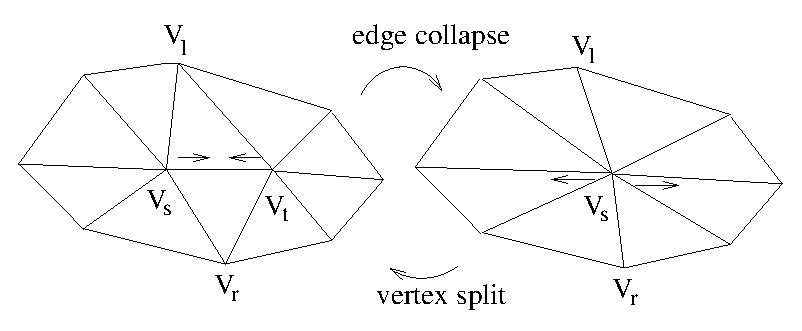
\epsfig{file = figures/split2.eps, height = 0.9in}
    \caption{Edge collapse and its reverse vertex split\label{model:split}}
    \end{minipage}
    \hspace{0.2cm}
    \begin{minipage}[b]{0.5\linewidth}
    \centering
    \epsfig{file = figures/dag1.eps, height = 1.2in}
    \caption{Dependency between vertex splits represented as a DAG.\label{model:dag2}}
    \end{minipage}
    \end{figure}

    %% Here we added the paragraph to justify the choice of the model
  Progressive meshes are well adapted for streaming since
  they offer the finest level of progressivity --
  it allows refinement at the granularity of vertices. 
  This progressivity is crucial for our
  application since a streamed vertex split only depends on
  the vertex splits that generated its neighbors, and not on other
  refinement operations of the same level (like for
  subdivision surfaces). Therefore, only dependencies among
  the vertex splits are crucial.

    Many extensions and variations to Hoppe's
    progressive mesh have been proposed (e.g.,
    \cite{614450,319358,383281,multiresolution:chen}).  The main idea
    behind these extensions is to combine multiple
    operations into one, thereby further reducing the
    redundancy and improving the efficiency. In particular, Pajarola and 
    Rossignac proposed a compressed progressive mesh (CPM) representation to reduce
    the size of a progressive mesh \cite{614450}. While this paper
    only considers the original progressive mesh, our
    model is general enough to model many of these
    extensions. 

    Significant differences exist between progressive mesh
    streaming and video streaming.  First, in video streaming,
    every packet should be received in time, or it will not
    be played back.  Hence, generally sending new data is more
    important than re-sending old data. On the contrary,
    in streaming of a progressive mesh, old data is
    usually more important than new one, since the
    reconstruction begins with the most significant refinement.
    Given this observation, retransmission of a lost packet is
    not only useful, but it should also take priority
    over transmission of new packets.

    Second, in progressive mesh, there is no strict order
    of vertex splits rendering order, unlike in video where
    frames must be displayed in sequence. A received vertex split
    can be rendered immediately as long as all the vertex splits
    it depends on have been received.  When a packet is lost, the
    subsequent received packets may still be decodable.  Those
    vertex splits received afterwards that depend on the
    lost packet, however, have to wait until the lost packet
    is retransmitted successfully before they can be displayed.
    This observation hinted that we should reduce the dependencies
    between packets as much as possible, since dependencies cause
    delay in rendering details generated by vertex splits.

    Third, a video frame is usually larger than a packet,
    causing the streaming application to split the video frame
    into several packets.  On the other hand, in progressive mesh,
    a vertex split is small (in the order of 10 - 15 bytes).  Thus,
    before the application transmits the mesh, it needs to group
    vertex splits into packets.   This \textit{packetization}
    process affects the dependencies among the packets, which in
    turn affects the delay in rendering if some packets are lost.
\\
\subsection{Related Work}
\label{s:model:related}

    Given the background in progressive mesh, we now describe
    related research in network transmissions of progressive mesh. 
    Three main classes of work exist 
    -- error resilient compression, error control, and
    packetization.

    Existing work in robust mesh compression aims to
    reduce dependencies among the mesh \cite{error:Park,error:Yan}.
    Similar to introducing key frames or restart marker in video/image
    coding, mesh
    segmentation is used to reduce the affected range of one
    packet loss. In robust mesh compression, a mesh is typically
    divided into several independent parts and then coded separately.
    Therefore the effect of one packet loss is confined to the part to which
    it belongs. The finer the partition is, the fewer the affected vertices
    are.  The coding efficiency, however, will decrease
    due to more redundancies and less correlation.

    Al-Regib and Altunbasak \cite{unequal:Al-Regib} proposed an
    unequal error protection method to improve the resilience of
    progressive 3D mesh based on CPM (compressed progressive meshes). Forward error
    correction (FEC) codes are added to the
    base mesh and additional levels-of-detail information to maximize 
    the decoded mesh quality.  The method is similar to FEC protection 
    of video data.
    As argued in the previous section, we believe that for streaming
    of 3D meshes, retransmission is always a better choice (except in
    cases such as multicast where retransmission is not scalable).
    Chen et al. \cite{chen05hybrid} also applied FEC to streaming
    progressive meshes. They analyzed several transmission schemes:
    TCP only, UDP only, TCP with UDP, and UDP with FEC, and studied
    their effects experimentally on the transmission time and decoded
    mesh quality.
    Al-Regib et al. proposed an application layer protocol, 3TP,
    for streaming of 3D models \cite{3tpregib}, combining both TCP 
    and UDP.  In 3TP, important packets are sent using
    TCP, while the rest are sent with UDP to minimize delay.

    
    Packetization of different model is tackled by
    Harris III and Karvets in \cite{harris:design}.   They proposed
    a protocol named On-Demand Graphic Transport Protocol (OGP)
    for transmitting 3D models represented as a tree of bounding volumes.
    A key component of the protocol is to decide which bounding volumes
    to send.  OGP begins with packing the largest possible subtree at
    the root and continues to pack the nodes in the subtree of
    acknowledged nodes in breadth-first order.  
    Gu and Ooi \cite{Gu:Packetization} were the first to look at
    the packetization problem for progressive meshes.  They model
    the packetization problem as a graph problem where the objective
    is to equally partition the graph into $k$ partitions with minimum
    cut size.  The problem is shown to be NP-complete and a heuristic
    is proposed.  They, however, assume that every vertex split is
    equally important.  In practice, the importance of vertex splits can
    vary considerably.  

    These existing studies are mainly concerned with dependencies
    (packetization and mesh segmentation) and importance
    of mesh data (unequal error protection and use of reliable protocol), 
    two factors that affect the quality of decoded meshes.  None, however,
    have looked at both factors and characterize 
    their effect on quality.  We aim at achieving this by proposing
    an analytical model.

\section{Analytical Model}
\label{s:model:model}
    We now develop an analytical model for transmission of
    progressive mesh over lossy networks.  We first need to model
    the progressive mesh and the network.  Since typically
    the base model is small (less than 1\% of the total size) 
    and is transmitted using reliable
    transport protocols \cite{3tpregib}, we assume that the
    base model has been received by the
    receiver. We will focus on modeling the vertex splits,
    which can be represented as a directed acyclic graph (DAG)
    (see Figure~\ref{model:dag2}). In the DAG, nodes represent
    the vertex split operations, and edges represent the dependency
    between these operations. We assign each node a weight,
    which corresponds to the importance of the vertex split.
    We will use the terms node and vertex split interchangeably
    in this paper.

    On the sender, vertex splits are grouped into packets,
    each containing equal number of vertex splits.  We say packet $P$ is a \textit{parent packet}
    of the vertex split $v$ if %the vertex split 
    $v$ 
    depends on at least one vertex split in $P$.  Therefore, a vertex split
    can be decoded only after the packet containing it and all its
    parent packets are received.

\if0
\begin{figure}
\centering
\epsfig{file = figures/dag1.eps, height = 1.2in}
\caption{Dependency between vertex splits represented as a DAG.\label{model:dag2}}
\end{figure}
\fi

    Let $B$ be the average
    sending rate\footnote{decided either by the available bandwidth or by TCP friendly requirement} and $p$ be the packet loss rate.
    In the model, we assume that packet losses are independent to each other for simplicity.
    In Section \ref{s:model:experiment}, we %will
    show that our model still works well under realistic packet losses (more bursty).
    We assume a retransmission-based protocol -- the sender resends a packet when its loss is detected.
    %a retransmission request (NACK) is sent back to the sender,
    %triggering a retransmission.  
    %the sender resends this packet. 
    Let $T_d$ be the
    average period between the time a packet %$P$ 
    is sent and the
    time %$P$'s 
    its loss is detected at the sender.
    %$T_d$ is the round trip time plus some constant.
    While $B$, $p$, and $T_d$ are likely to varies in practice during to network dynamics, 
    we adopt a common technique in performance modeling by constructing our model using 
    their average values and assuming that they are constants.
    We study the effects of this assumption in Section \ref{s:model:experiment}.

    We discretize time into slots.  Each slot is the time to
    send one packet.  Thus, one time unit is $L/B$ seconds, where $L$ is the
    packet size.  
    The time $T_d$ is normalized to this
    time unit.  Thus, $T_d$ can also be interpreted as the number
    of packets transmitted between sending a packet $P$ and detecting
    the loss of $P$.  Moreover, at the sender,
    we define the time the first packet is sent as time $0$, whereas, at
    the receiver, we define the time the first packet is received (if it
    is not lost) as $0$.  Therefore, a packet sent at time $t$ will be 
    received at time $t$ if it is not lost.  Thanks to the different 
    timeline at the
    receiver, we avoid an additional term, $RTT/2$, in
    equations related to the received time and decoded time. 
    We denote the $i$-th packet sent (and not retransmitted) as $P_i$, where $i = 0, 1, ...$.
    Table~\ref{t:model:notation} summarizes these notations as well as
    other major notations used in this paper.

% NOTATION

    \begin{table}
    \begin{centering}
    \begin{tabular}{|r|l|}
    \hline
    $L$ & packet size \\
    $B$ & sending rate \\
    $p$ & packet loss rate \\
    $T_d$ & time between sending a packet and \\
          & receiving its NACK\\
    $S_i$ & sending time of $P_i$ (wrt. sender time)\\
    $R_i$ & received time of $P_i$ (wrt. receiver time)\\
    $D_j$ & the time vertex split $j$ is decoded at the receiver \\
    $w_j$ & the importance of vertex split $j$ \\
    $N_{d,t}$ & number of packets decoded at time $t$ \\
    $N_{r,t}$ & number of packets received at time $t$ \\
    $\Delta_t$ & increase in expected number of decodable packet at time $t$\\
    \hline
    \end{tabular}
    \caption{Notations used in our model\label{t:model:notation}.}
    \end{centering}
    \end{table}

    With that background, we are able to explain how we obtain the
    expected value of sending time, received time, and decoding time
    of a vertex split.
\if\showproof0
    Due to space constraints, we will only sketch the proofs in this
    paper.
\fi

\subsection{Sending Time and Receiving Time}
%\newtheoremstyle{definition}
Let $S_i$ be the time when $P_i$ is sent. %If $k$ packets have been lost and retransmitted before $S_i$ then packet $i$ is sent at time $S_i=i+k$. Lemma~\ref{theorem_ts} computes the probability of this event and the expected value $E[S_i]$ of the time when the packet $i$ is sent.
Lemma~\ref{model:theorem_ts} computes the distribution of $S_i$ and the expected value $E[S_i]$.
\begin{lemma} \label{model:theorem_ts}
If $i \geq T_{d}$, %then for any $k \geq 0$,
\begin{eqnarray*}
E[S_i]          &=& (i - T_d + 1)\frac{1}{1-p} + T_d - 1.
%$E[S_i]          = (i - T_d + 1)\frac{1}{1-p} + T_d - 1$.
\end{eqnarray*}
%Pr(S_i = i+k)     &=& \binom{i-T_d+k}{k}p^k(1-p)^{i-T_d+1}\\
%ooiwt - no need pdf in the lemma since not using it elsewhere.
Otherwise, %if $i < T_d$, then 
$S_i = i$.
\end{lemma}
\if\showproof1
\begin{proof}
    If $i<T_d$, then $S_i = i$ since no retransmission exists.
    Now we consider the case when $i \geq T_d$.
    The number of transmissions before one successful transmission
    is a random variable with geometric distribution and its
    expected value is $1/(1-p)$.  Therefore, the expected value of
    total transmissions after time $T_d$ when there are
    $i - T_d + 1$ known successful transmissions is $(i - T_d +1)/(1-p)$.
    Hence, we have 
    %\begin{displaymath}
        $E[S_i]          = (i - T_d + 1)\frac{1}{1-p} + T_d - 1$.
    %\end{displaymath}
    %Between time $0$ and time $i+k$ there are $i+k+1$ time slots.
    %Among them, $i+1$ slots are used to send new packets (packet $0$
    %to packet $i$) and $k$ slots are used for retransmissions.
    %Retransmissions cannot happen before time slot $T_d$ because the earliest
    %time to detect a packet loss is $T_d$. Moreover, time slot
    %$i+k$ is used to send the new packet $i$. Hence, the $k$ retransmissions
    %only happen in $i+k-T_d$ time slots 
    %(from time slot $T_d$ to time slot $i+k-1$), so there are in total
    %$\binom{i-T_d-k}{k}$ possible situations. 
    %
    %Since packet $i$ is sent at time $i+k$, $i+1$ slots are used for
    %sending new packets and $k$ are used for retransmissions.
    %Retransmissions cannot happen at the first $T_{d}$ slots (no packet
    %loss can be detected before time $T_d$), and the time slot $i+k$ is
    %used for transmission of new packet $i$. 
    %Therefore, the $k$ retransmissions can only happen between $T_d$ and
    %$i+k-1$, in total $i-Td+k$ slots. 
    %Moreover, 
    % 
    %%Time slot $t$ is used for retransmission if and only if the packet sent
    %%at time $t-T_d$ is lost, so the probability for a time slot to be used
    %%for retransmission is also $p$. From $T_d$ to $i+k$, $k$ time slots
    %%are used for retransmissions and $i-T_d+1$ time slots are used to send
    %%new packets. Therefore, for each possible situation,
    %%the probability is $p^{k}(1-p)^{i-T_d+1}$.
    % 
    %A retransmission corresponds to a packet loss happens $T_d$ before,
    %so a slot. 
    %Therefore, among the $i+k-T_d+1$ time slots from $T_d$ to $i+k$, 
    %a time slot is used for retransmission in probability $p$ and 
    %sending new packet in probability $1-p$. 
    %Since the time slot $i+k$
    %is used to send packet $i$, so the $k$ retransmissions can only
    %happen in the rest $i-T_d+k$ time slots.
    %
    %%Hence, we have
    %%\begin{displaymath}
    %%Pr(S_i = i+k)     = \binom{i-T_d+k}{k}p^k(1-p)^{i-T_d+1}.
    %%\end{displaymath}
    %
    %%The number of transmissions before one successful transmission
    %%is a random variable with geometric distribution and its
    %%expected value is $1/(1-p)$.  Therefore, the expected value of
    %%total transmissions after time $T_d$ when there are
    %%$i - T_d + 1$ known successful transmissions is $(i - T_d +1)/(1-p)$.
    %%Hence, we have 
    %%\begin{displaymath}
    %%    E[S_i]          = (i - T_d + 1)\frac{1}{1-p} + T_d - 1.
    %%\end{displaymath}
    \end{proof}
\else
    % Proof sketch
    %\textbf{Proof sketch}
    
    \begin{proof}
    Whether a packet is sent successfully or not can be known only after $T_{d}$.  
    At time $i + k$ ($k \geq 0$),  the result of first $i + k - T_d + 1$ transmissions are
    known (we call them \textit{known transmissions}), but the result of the following $T_d - 1$
    transmission remains unknown (we call it \textit{unknown transmission}).  For $t \geq T_d$,
    a new packet is sent at $t$ only when the
    transmission at $t-T_d$ is known to be successful.  Hence, if packet $i$ is sent at
    $i+k$, then among the $i + k - T_d + 1$ known transmissions, $i - T_d + 1$
    transmissions are successful and $k$ transmissions fail.
    The variable $k$ has a negative binomial distribution,
    and the expression for $Pr(S_i = i+k)$ follows.
    \end{proof}

    The total number of transmissions until a packet is successfully sent is
    a random variable following geometric distribution with expected value of
    $1/(1-p)$. Therefore, the expected value of total transmission number
    until $i - T_d + 1$ packets are successfully sent is $(i-T_d+1)/(1-p)$.
    Including the subsequent $T_d - 1$ unknown transmissions, we have the expression
    for $E[S_i]$.  \QED
\fi

    
Let $R_i$ denote the time a packet $i$ is received.
The probability that a packet $i$ is received at time $t$
is given as follows.
\begin{lemma}
\label{l:model:preqt}
  \begin{equation*}
    Pr(R_i = t) = \left\{
   \begin{array}{ll}
    (1-p)p^{n_{i,t}} & \mbox{if } (t-S_i) \mod T_d = 0  \\
        0                & \mbox{otherwise}
   \end{array}
   \right.
\end{equation*}
    where $n_{i,t}=\lfloor(t - S_i)/T_d\rfloor$ is the number of times packet $i$ was lost when $R_i = t$.
\end{lemma}

    %\textbf{Proof sketch}
    \begin{proof}
    The lemma follows from the fact that a packet can only be
    received at a time that is a multiple of $T_d$ after the
    first time it was sent. %\QED
    \end{proof}

    Note that here $S_i$ is a random variable but we approximate
    the decoding time by using the expected value of $S_i$ computed
    from Lemma~\ref{model:theorem_ts}.  This approximation is accurate
    enough (as shown in the next subsection) as long as the variance
    of $S_i$ is small.
    %\footnote{This approximation
    %leads to the possibility of two packets arriving at exactly
    %the same time.  In this case, we break ties by randomly reordering
    %the arrival of the packets}.

\begin{lemma}
\label{l:model:prlet}
\begin{equation*}
Pr(R_i \leq t) = 1 - p^{n_{i,t}+1}.
%$Pr(R_i \leq t) = 1 - p^{n_{i,t}+1}$.
\end{equation*}
\end{lemma}

    %\textit{Proof sketch}
    \begin{proof}
    A packet is received strictly after time $t$ if and only if the packet
    is lost at least $n_{i,t}+1$ times and the probability is
    $p^{n_{i,t}+1}$. 
    %Given $t$, the probability that a packet is received strictly after
    %time $t$ is the same as the probability that the packet has been
    %lost $n_{i,t} + 1$ times, or $p^{n_{i,t}+1}$.  
    Lemma~\ref{l:model:prlet} follows. %\QED
    \end{proof}

\subsection{Decoding Time of a Vertex Split}

    Once we expressed both sending time and receiving time,
    we can approximate the decoding time of a vertex split $v$, denoted
    as $D_v$.

    Let $\mathcal{P}(v)$ be the set of
    all parent packets of the vertex split $v$ and the packet including $v$, then the
    probability that vertex split $v$ can be decoded at time $t$
    is given by the probability that one of the packet in $\mathcal{P}(v)$
    is received at time $t$ and all other packets in $\mathcal{P}(v)$
    is received before time $t$.
    \begin{eqnarray}
    \label{e:model:pdvt}
        Pr(D_v = t) = \sum_{i \in \mathcal{P}(v)} \frac{Pr(R_i = t)}{Pr(R_i < t)} \prod_{k \in \mathcal{P}(v)} Pr(R_k < t).
    \end{eqnarray}

    Lemma~\ref{l:model:preqt} and \ref{l:model:prlet} give the expression
    for $Pr(R_i=t)$ and $Pr(R_i<t)$ respectively.
    Once we have the probability distribution of $D_v$, we can
    estimate the expected decoding time of a vertex split $v$
    with
    \begin{equation}
    \label{e:model:e_et}
        E[D_v] = \sum_{j=t}^{\infty}jPr(D_v = j).
    \end{equation}

    Since the probability $Pr(D_v = t)$ decreases exponentially
    as $t$ increases, in practice we can numerically estimate the
    expected decoding time by considering only the first few
    terms of the sum.  In this paper, we consider $j$ from $S_i$ to $S_i + 3T_d$,
    which we found to be accurate enough for practical purposes.
    That is,
    a packet is considered to be lost at most three times in a row.
    For larger loss rate, one can consider more terms to trade-off
    computation time and accuracy.


    Our analytical model is useful in several ways.  
    These equations can help us in understanding the effect of dependency (see Section \ref{s:model:effect}) when transmitting 
    a progressive mesh over a lossy network.  Our model can lead to some simple close form equations in two special cases.  
    We can also compute the expected decoded quality analytically, leading to a faster alternative to 
    simulation (see Section \ref{s:model:analytical_quality}) as a way to evaluate the effects of network conditions on
    progressive mesh streaming.
    Moreover, a better packetization algorithm can be designed based on this analytical model (Section \ref{s:model:scheduling}). 
    We introduce these applications of our model next.


\section{Effects of Dependencies}
\label{s:model:effect}

    This section discusses the effects of dependencies
    on the number of decodable packets, as a function of
    $p$ and $T_d$.  As mentioned in Section~\ref{s:model:mesh},
    packetization at the sender may affect
    decoded mesh quality.  We quantify 
    this effect by estimating the number of
    decodable packets at a given time for two extreme cases
    of dependencies.  The effects of any other dependency
    will be bounded by what we obtained for these two extreme cases.

    In the first case (ideal
    case), there is no dependency among packets.
    In the second case (worst case), a packet depends on all other packets
    sent previously.  Note that these two dependency models are
    independent of any packetization scheme.
    Moreover, we are computing the number of decodable \textit{packets} rather
    than \textit{vertex splits}.  This simplification does not affect
    the accuracy of our model
    since in the ideal case, we can assume that all vertex splits
    in a packet are decodable as soon as the packet is received (no dependencies
    among packets).  In the worst case, if a packet's dependency is not
    satisfied, then all vertex splits contained in that packet are
    not decodable.  Thus, the number of decodable packets is
    proportional to the number of decodable vertex splits in these two extreme
    cases.

    Let $N_{r,t}$ be the number of received packets at time $t$ and
    $N_{d,t}$ be the number of decoded packets at time $t$.   We show
    how to compute the expected value of $N_{d,t}$ for the two
    extreme cases in the next two subsections.

\subsection{Ideal Case}
\begin{theorem}
\label{t:model:ideal}
    In the case with no dependencies among the packets,
    \begin{eqnarray*}
%    Pr(N_{r,t} = k) &=& \binom{t+1}{k}p^k(1-p)^{t+1-k},\\
    E[N_{r,t}] &=& E[N_{d,t}] = (t+1)(1-p).
    \end{eqnarray*}
\end{theorem}
    %\textbf{Proof Sketch}
    \begin{proof}
    In the ideal case, each packet can be decoded independently
    regardless of other packets.  Thus, at any time $t$,
    $N_{d,t} = N_{r,t}$.
    Let $a_i$ represents the result of a transmission at time $i$,  
    that is
    \begin{displaymath}
    a_i = \left\{\begin{array}{ll}
    1 & \textrm{if transmission is successful}\\
    0 & \textrm{if transmission is failed}\\
    \end{array}\right.
    \end{displaymath}
    The expected number of successful transmissions at time $t$ is
    \begin{eqnarray*}
    E\big[\sum_{i=0}{t}a_i\big] = \sum_{i=0}{t}E[a_i] = \sum_{i=0}{t}(1-p) = (t+1)(1-p)
    \end{eqnarray*}
    %The number of successful transmission at time $t$ is equivalent to
    %the number of successful Bernoulli trials out of $t+1$
    %transmission\footnote{recall that the first transmission is at time 0}.
    %Theorem~\ref{t:ideal} follows.
    %\QED
    \end{proof}

\subsection{Worst Case}

    

    In the worst case, a packet depends on all previous packets (packets
    with smaller index).  The expected number of packets decodable at
    time $t$, is given by the following equation:
    \begin{eqnarray}
    \label{e:model:endt}
    E[N_{d,t}] = \sum_{i=0}^{m} \prod_{j=0}^i Pr(R_j \le t),
    \end{eqnarray}
    where $m$ is the total number of packets\footnote{When $p=0$, $N_{d,t}$ is always $t+1$.  We assume non-zero $p$ in this section.}.

    Obtaining a close form formula for $E[N_{d,t}]$ is more tricky.
    
    We therefore first derive a close form formula for $\Delta_t$, which is 
    the increase of the expected number of packets decodable at time $t$,
    that is, $\Delta_t = E[N_{d,t}] - E[N_{d,t-1}]$. 
    We let $\Delta_0$ be $(1-p)$ since
    the expected number of packets decodable at time 0 is $(1-p)$.

    Suppose $P_0$ is successfully received at time $0$.  We remove $P_0$
    from the dependency graph, reducing the dependency graph to a 
    graph with the same dependency structure
    but with one less packet.  The expected number of decodable
    packets from time $1$ to time $t$ is the same as the expected
    number of decodable packets from time $0$ to time $t-1$.  Therefore,
    when $t>0$, we have
    \begin{eqnarray}
    \label{e:model:p0received}
    E[N_{d,t}|_{\textrm{$P_0$ received}}] - E[N_{d,t-1}] &=& 1.%\\
    %\Delta_t|_{\textrm{$P_0$ received}} &=& 1.
    \end{eqnarray}
    %when $t>0$.

    Now consider what happens if $P_0$ is lost in its first transmission. 
\begin{figure}[htbp]
\centering
\epsfig{file = figures/comparison.eps, height = 1.5in}
\caption{If packet $0$ is lost, compared with the transmissions begin from time slot 1, only the sending order of first $T_d$ packets is different.}\label{f:model:comp}
\end{figure}
    $P_0$ will be retransmitted at time $T_d$. If we view time $t=1$ as
    the new starting time of transmission, then the only difference between the new
    sending order and the original one is that in the new sending order, $P_0$ is
    sent at time $T_d-1$ and $P_1$ to $P_{T_d-1}$ will be 
    sent one slot earlier (see Figure~\ref{f:model:comp}). The sending time 
    and receiving time of other packets will be the same. 
    Therefore we have:
    \begin{eqnarray}
    \label{e:model:p0notreceived}
        Pr(R_i \le t|_\pOlost)= \left\{\begin{array}{ll}
        Pr(R_{T_d-1} \le t-1)             & \textrm{if $i = 0$}\\
        Pr(R_{i-1}   \le t-1)             & \textrm{if $1 \le i \le T_d - 1$}\\
        Pr(R_i       \le t-1)             & \textrm{if $i \ge T_d$} \\
        \end{array}\right.,
    \end{eqnarray} 
    and hence
    \begin{eqnarray}
    \label{e:model:equal}
       \prod_{i=0}^{m}Pr(R_i \le t|_\pOlost) = \prod_{i=0}^{m}Pr(R_i \le t-1) & \textrm{for any $n \ge T_d$},
    \end{eqnarray}
    where $m$ is the total number of packets.
    %Also, we note that 
    %\begin{eqnarray}
    %\label{e:zero}
    %   Pr(R_t \le t|_\pOlost) = 0
    %\end{eqnarray}

    Moreover, from Lemma~\ref{l:model:prlet}, we have the following Lemma: 
    \begin{lemma}
    \label{l:model:recv_td}
    At time $t = nT_d$, we have
    \begin{eqnarray*}
    Pr(R_i \leq t - 1) = 1 - p^n \textrm{when $0 \leq i \le T_d$.}
    \end{eqnarray*}
    At time $t = nT_d + b$ and $b>0$, we have
    \begin{eqnarray*}
        Pr(R_i \le t-1) = \left\{\begin{array}{ll}
        1 - p^{n+1} & \textrm{when $0 \le i < b$}\\
        1 - p^n     & \textrm{when $b \le i < T_d$ }\\
        \end{array}\right.
    \end{eqnarray*}
    \end{lemma}
    \begin{proof}
    The sending time of packet $i$ ($ 0 \leq i \le T_d$) 
    is always $i$ (recall that the time unit is the time to transmit a packet). Before time $nT_d$, 
    they all have $n$ chances to be transmitted, and the probability to
    be received before time $nT_d$ is $1 - p^n$.
    At time $nT_d + b$ and $b >0$. The packet $0$ to packet $b-1$ will
    have $n+1$ chances to be transmitted, therefore the probability to be
    received before time $nT_d + b$ is $1 - p^{n+1}$. The others have only
    $n$ chances to be transmitted, and hence the probability to be
    received before time $nT_d + b$ is $1-p^n$. 
    \end{proof}

    Then we can prove the following lemma:
    \begin{lemma}
    \label{l:model:p0lost}
    \begin{eqnarray*}
    E[N_{d,t}|_\pOlost] - E[N_{d,t-1}] = \dfrac{p-1}{p}(1-(1-p^{n+1})^b) \\
    \textrm{where $t = nT_{d}+b > 0$ and $n,b \in\mathbb{Z^+}; 0 \le b<T_d$.}
    \end{eqnarray*}
    \end{lemma}
    \begin{proof}
    \begin{align*}
     &E[N_{d,t}|_\pOlost] - E[N_{d,t-1}] & \\
    =& \sum_{i=0}^{m}\prod_{j=0}^{i}Pr(R_{j} \le t|_\pOlost) - \sum_{i=0}^{m}\prod_{j=0}^{i}Pr(R_{j} \le t-1) & 
        \text{(from Eqn. \ref{e:model:endt})} \\
    =& \sum_{i=0}^{T_d - 1}\big[\prod_{j=0}^{i}Pr(R_{j} \le t|_\pOlost) - \prod_{j=0}^{i}Pr(R_{j} \le t-1)\big] &
        \text{(from Eqn. \ref{e:model:equal})}\\
    =& \sum_{i=0}^{T_d - 1}\big\{[Pr(R_{T_d-1} \le t-1) - Pr(R_{i} \le t-1)]\prod_{j=0}^{i-1}Pr(R_{j} \le t-1)\big\} 
        & \text{(from Eqn. \ref{e:model:p0notreceived})}\\
    \end{align*}

    We now consider two cases.  First, suppose $b = 0$.  From Lemma~\ref{l:model:recv_td}, the receiving probability of 
    all packets from 0 to $T_d - 1$ are the same. So $[Pr(R_{T_d-1} \leq t-1)
    - Pr(R_i \leq t-1)]$ is always 0 and hence $E[N_{d,t}|_\pOlost] - E[N_{d,t-1}] = 0$. 
    Since $\dfrac{p-1}{p}(1- (1-p^{n+1})^b) = 0$ when $b = 0$, the lemma holds.

    Now, consider the case where $0 < b < T_d$.
    From Lemma~\ref{l:model:recv_td}, packet $0$ to packet $b-1$ has $n+1$ chances to
    be transmitted, while packet $b$ to packet $T_d - 1$ has $n$ chances to
    be transmitted. Therefore, 
    \begin{align*}
     &E[N_{d,t}|_\pOlost] - E[N_{d,t-1}] & \\
    =&\sum_{i=0}^{b-1}[(1-p^{n})-(1-p^{n+1})](1-p^{n+1})^{i} = \dfrac{p-1}{p}(1- (1-p^{n+1})^b) \\
    %=& \dfrac{p-1}{p}(1- (1-p^{n+1})^b)\\
    \end{align*}
    Hence, the lemma still holds in this case.
    \end{proof}
    
    Combining the results in this section, we have the following:
    %\begin{theorem}
    \begin{lemma}
    %\label{t:worst}
    \label{l:model:worst}
    %\[
        %\Delta_t = (1-p)(1-p^{n+1})^b,
        $\Delta_t = (1-p)(1-p^{n+1})^b$,
    %\]
where $t=nT_d+b$ and $n,b\in\mathbb{Z^+}; 0 \le b<T_d$.
    %\end{theorem}
    \end{lemma}
    \if\showproof1
    \begin{proof}
    \begin{align*}
    %\Delta_t &= (1-p)\Delta_t|_\textrm{$P_0$ received} + p\Delta_t|_\pOlost \\
    \Delta_t &= (1-p)E[N_{d,t}|_\textrm{$P_0$ received}] + pE[N_{d,t}|_\pOlost]
    - E[N_{d,t-1}]\\
             &= (1-p)\{E[N_{d,t}|_\textrm{$P_0$ received}] - E[N_{d, t-1}]\} 
             + p\{E[N_{d,t}|_\pOlost] - E[N_{d, t-1}]\}\\
    \intertext{when $t>0$, from Eqn \ref{e:model:p0received} and Lemma~\ref{l:model:p0lost}}
             %&= (1-p) + (p-1)(1-(1-p^{n+1})^b) \\
             %&= (1-p)(1-p^{n+1})^b.
             &= (1-p)+(p-1)(1-(1-p^{n+1})^b)=(1-p)(1-p^{n+1})^b.
    \end{align*}
    when $t=0$, the above formula still holds because $\Delta_0 = 1-p$.
    \end{proof}
    \fi

    Then, finally we could obtain $E[N_{d,t}]$ as
    follows:
    \begin{theorem}
    \label{t:model:worst}
    %if $t < T_d$ then
    %\[
    \begin{eqnarray*}
       \textrm{if $t<T_d$ then, } E[N_{d,t}] &=& (1-p)\Big[\dfrac{1-(1-p)^{t+1}}{p}\Big]\\ 
    %\]
    %else 
    %\[
       \textrm{else, } E[N_{d,t}] &=& (1-p)\Big\{\sum_{i=1}^n\Big[\dfrac{1-(1-p^i)^{T_d}}{p^i}\Big] +
       \dfrac{1-(1-p^{n+1})^{b+1}}{p^{n+1}}\Big\}
    %\]
    \end{eqnarray*}
    where $t=nT_d+b$ and $n,b\in\mathbb{Z^+}; 0 \le b<T_d$.
    \end{theorem}
    %\textbf{Proof sketch}
    \begin{proof}
    We have $E[N_{d,t}] = \sum_{i=0}^{t}\Delta_t$, and from Lemma~\ref{l:model:worst}, we
    find that the $\Delta_t$ during each $T_d$ is a part of geometric series. From
    $\sum_{i=0}^nq^i = \dfrac{1-q^{n+1}}{1-q}$, we can prove this theorem.
    \end{proof}

\subsection{Insights}
    We have derived the expected decodable number of packets for
    two cases of dependencies: the ideal case where there are no
    dependencies between the packets, and the worst case, where
    a packet always depends on previously sent packets.  Any
    packetization algorithms will lead to a
    dependency structure between the packets that lies between
    these two extreme cases.  The difference between the number of
    decodable packets for these two cases therefore gives us an
    indication of how much improvements we can get if we intelligently
    group the vertex splits into packets.  
    
    The next question is how big is the
    gap between the two extreme cases.
    Let $f(i)$ be the difference of average decodable number of packets in time $iT_d$. Then
    from Theorem \ref{t:model:ideal} and Theorem \ref{t:model:worst}, we have
    \begin{eqnarray*}
    f(1)         &=& (1-p)T_d - (1-p)\frac{1}{p}[1-(1-p)^{T_d}]\\
        f(i)-f(i-1)  &=& (1-p)T_d - (1-p)\frac{1}{p^i}[1-(1-p^i)^{T_d}],
    \end{eqnarray*}
    where $i \geq 1$. After some mathematical manipulations, we have
    \begin{eqnarray*}
    f(i) - f(i-1) &=& (1-p)\sum_{j=2}^{T_d}\Big[(-1)^j\binom{T_d}{j}p^{(j-1)i}\Big];\\
    f(i)          &=& (1-p)\sum_{j=2}^{T_d}\Big[(-1)^{j}\binom{T_d}{j}\sum_{k=1}^i p^{(j - 1)k}\Big];\\
    f(\infty)     &=& (1-p)\sum_{j=2}^{T_d}\Big[(-1)^{j}\binom{T_d}{j}\frac{p^{j-1}}{1-p^{j-1}}\Big]\\
                  &\leq& \sum_{j=2}^{T_d}\Big[\binom{T_d}{j}\frac{(-p)^{j}}{p}\Big] = \frac{1}{p}[(1-p)^{T_d} -1 + T_{d}p]\\
    %              &=& \frac{1}{p}[(1 - p)^{T_d} - 1 + T_{d}p]
    \end{eqnarray*}
    Therefore, we can see the difference is upper-bounded.
    Since when $p$ is small, $\sum_{k=1}^i p^k$ converges to $\frac{p}{1-p}$ quickly,
    so the difference after 2 to 3 $T_d$ is already very close to the upper-bound value.
    
    
    The main observation from our analysis is that \textit{
    dependencies matters only during the first few $T_d$s.}
    In Theorem~\ref{t:model:worst}, if $t$ is large, and $p$ is small
    enough, then the factor $1-p^{n+1}$ tends to 1.  Hence, as
    time progresses, the increase in number of decodable packets
    for the worst case becomes close to $1-p$ for each time slot.
    If we plot two curves, showing expected number of decodable
    packets versus time, for the ideal and worst case, then the
    two curves become almost parallel for large values of $t$.  In fact,
    if we consider the difference between the curve at time $xT_d$,
    then the difference tends to a constant that depends only on
    $T_d$ and $p$ as $x$ tends to infinity.
    Figure~\ref{model:extreme} shows an example of such two curves, with
    $p = 0.1$ and $T_d = 40$.

    This observation leads us to believe that optimization of
    packet dependencies only matters during the first few $T_d$s. 
    After that, the dependencies among the packets will not affect
    the number of decodable packets.  Further, in progressive mesh,
    the importance of the vertex splits decreases as the model becomes
    incrementally refined.  Thus, the contributions of the later vertex
    splits to the decoded quality of the mesh are less than the contribution
    of previous vertex splits.

    This observation is good news -- regardless of how large the
    progressive mesh is, only dependencies among vertex splits sent during the
    first few $T_d$s matter.  Thus, any packetization
    algorithm only needs to focus on the vertex splits sent during
    this initial period, reducing the computational costs significantly.

\begin{figure}[htbp]
\centering
\epsfig{file = figures/extreme40_1.eps, height = 2.5in, angle = 270}
\caption{The number of decodable packets for ideal case and worst case. $T_d= 40$, Loss rate $p =0.1$. In the figure, we assume the first packet arrives at time 1.}\label{model:extreme}
\end{figure}

%including what is maximum delay. Hong long is the critical range, in which the optimization is meaningful.

\section{Improving Mesh Quality}
\label{s:model:quality}
    Using our analytical model, we can now analytically compute the
    expected decoded mesh quality given the dependencies among %the
    vertex splits and %the order the packets are sent.
    the sending order of the packets.
    We first explain how we measure the
    quality of a progressive mesh.
\subsection{Expected Decoded Mesh Quality}
\label{s:model:analytical_quality}
    The quality of a simplified mesh represents how close it
    is compared to the original mesh. Some objective
    metrics have been proposed. Many of them are based on the
    Hausdorff distance between a set of sample points on the original
    mesh and the corresponding ones on the simplified one.
    For example, Metro \cite{cignoni98metro} and M.E.S.H \cite{mesh:aspert}
    can be used to obtain both the mean and the maximum face to face distances
    between two models.
    %\cite{cignoni98metro}.

    %Some survey needed here.
    In the case of a progressive mesh, the base mesh has the
    lowest quality, and each vertex split increases the
    quality by a certain amount. We define the \textit{importance} of
    a vertex split as the  increase in decoded mesh
    quality due to this vertex split.  
    This value can be determined by comparing the quality
    of the model before and after the vertex split operation.
    Strictly speaking, the importance value may depend on the split order,
    but, for simplicity, we assume that a refinement
    always improves the quality of the model by a value,
    independently of other refinements.  Then, the quality of a
    received model at time $t$ (or, \textit{intermediate
    quality}) can be represented as the summation of
    importance of all vertex splits decodable at $t$.
    Since the simplification process typically prefers collapsing an edge with low
    quality loss, edges with lower importance are collapsed earlier during the
    simplification and split later during the reconstruction.  Therefore, in 
    a progressive mesh, vertex splits operations are typically performed in 
    decreasing order of importance.

    This model of decoded mesh quality is general -- one can
    define different importance metric for a vertex split depending
    on how mesh quality is measured.
    %on the objective metric.  \todo{not so clear what the objective metric is here}. 
    For instance, if the mesh quality is view dependent, one
    can set the importance of a vertex split to zero if the vertex
    split is outside of the user's viewpoint \cite{258843}. 


    In progressive streaming, the quality of the mesh on the receiver
    increases over time, and plotting this quality versus time gives us
    a \emph{quality curve}.  
    We evaluate and compare different streaming strategies 
    of the same progressive mesh by comparing the quality curve.
    Because vertex splits contribute differently
    to the quality, the quality curve depends on the decoding time and decoding order
    of the vertex splits. %Therefore, decoding time of each vertex split
    %is needed in deciding the quality curve.
    %\todo{Is the last sentence not redundant: what differ between decoding time and
    %decoding order since time unit is a tick between receiving 2 packets?}
 
    %We evaluate and compare different streaming strategies of the
    %same progressive mesh
    %by examining the intermediate quality.  Note that as long as
    %the sending rate is the same, the complete mesh will be
    %received at the same time.  We are more interested in
    %intermediate quality, since in progressive transmission,
    %we want the users to view a mesh with the best possible quality
    %before the whole mesh is transmitted.  This intermediate
    %quality is important especially in interactive applications,
    %where what a user sees initially matters.

    Now we explain how our model can be used to estimate the quality 
    curve. The quality at time $t$ is the sum of importance of 
    decoded vertex splits. That is
    \begin{displaymath}
    q_t =  \sum_i w_i, \textrm{for all vertex split $i$ decoded before or at time $t$}.
    \end{displaymath}
    We define $s_i$ such that
    $s_i = 0$ if vertex split $i$ is not decoded yet at time $t$, and
    $s_i = 1$ if vertex split $i$ is already decoded at time $t$.
    Suppose we have $n$ vertex splits in total.
    Then we have
    %\begin{eqnarray*}
    %q_t    &=& \sum_{i=0}^{n}s_{i}w_{i}\\
    %E[q_t] &=& \sum_{i=0}^{n}w_{i}E[s_{i}] = \sum_{i=0}^{n}w_{i}Pr(D_i \leq t)\\
    $q_t    = \sum_{i=0}^{n}s_{i}w_{i}$, so
    $E[q_t] = \sum_{i=0}^{n}w_{i}E[s_{i}] = \sum_{i=0}^{n}w_{i}Pr(D_i \leq t)$.
    %       &=& \sum_{i=0}^{n}w_{i}Pr(D_i \leq t)
    %\end{eqnarray*}
    Since $Pr(D_i \leq t)$ can be obtained from Equation \ref{e:model:pdvt}, we are able to compute $E[q_t]$. 
    Therefore, we can evaluate a sending order by predicting the expected
    quality curve with our analytical model given the network condition
    and the mesh property. Moreover, in next section, we introduce that
    the predicted quality can also be used in designing streaming strategies, 
    particularly, packetization of vertex splits.

\subsection{A Packetization Algorithm}
\label{s:model:scheduling}

%    Recall that $T_d$ is
%    the time between sending a packet and detecting its loss at 
%    the sender, expressed in units of a packet transmission time.
%    If we assume a typical RTT of 250 ms, a packet size of 1500 bytes,
%    and a sending rate of 1.5Mbps, then the value of $T_d$ is 30.  With a
%    5\% loss rate, the gap between the two cases is about 15 packets.
%%    If we have about 100 vertex splits in each packet, then there is a
%%    1500 vertex splits difference between the two cases, which is significant.
%    The gap, however, decreases if the sending rate is
%    smaller or RTT is smaller ($T_d$ decreases).  The gap also decreases
%    when $p$ decreases.

%    During our experiments, we have observed instances with 
%    significant quality differences in the
%    rendered mesh with the same packet dependencies, with some 
%    instances giving much worse quality than what would
%    be predicted by the analysis in Section \ref{s:effect}.
%    The reason %for this mismatch 
%    is that our model analyzes the average behavior and gives us the
%    \textit{expected} number of decodable packets.  %Therefore, the
%    %average quality of the decoded mesh over a large number of
%    %streaming sessions will not differ too much.  
%    But, the
%    \textit{variance} for the number of decodable packets can be
%    large.  Thus, a viewer who receives a progressive 3D mesh
%    stream (a single sample) might still observe a significant
%    difference initially with different packet dependencies.
%    This fact motivates us
%    to apply our model to reduce the dependencies among packets splits during 
%    streaming of progressive meshes during the \textit{packetization} process.

Packetization refers to the process of grouping vertex splits into packets
before transmitting them over the network.  Due to dependencies among nodes,
packetization may introduce dependencies among packets (if a vertex split and
its parent are packed in different packets).  Therefore dependencies
affect the decoding time of the vertex splits and the intermediate quality of the
decoded model.  The intermediate quality of the rendered model can be 
important in interactive applications, especially during the initial stage of
streaming, since users may need to react to what they see quickly.

To improve the intermediate quality of the decoded model, we need to consider two
factors in the packetization: the importance of each vertex split, or node,
and the dependencies among nodes.  One strategy is to always send the most
important node first; the other is to packetize the packets to minimize its
dependency \cite{Gu:Packetization}.   If there is no packet loss, 
these two objectives can be achieved at the same time.  Since the vertex split operations
in a progressive mesh are typically executed in the decreasing order, we can simply
send the vertex splits in the first-in-first-out (FIFO) order, in the reverse order
of the edge collapse operations.  Since a node's parent packets are
always sent before the packet containing the node, a node can be decoded as
soon as it is received.  When packet loss exists, however, there is a conflict
between maximizing importance and minimizing dependencies.
FIFO satisfies the first objective, but may increase dependency among packets;
whereas to reduce dependency, one may send a node with lower importance
before a more important node. To trade-off between these two
objectives, we need to know the exact effect of both factors. In this section,
we show how we use our model developed in Section~\ref{s:model:model} to
help us select which node to pack.

    Before introducing our method called greedy, 
    we need to quantify the quality at 
    a given time $t$. 
    %One simple metric is to compare the intermediate quality at
    %a given time $t$; the other is to compare the time it 
    %takes for two streaming strategies to reach a given
    %intermediate quality.  These simple metrics are
    %nonetheless too restrictive.  
    Simply comparing the %intermediate 
    quality at time $t$ 
    %or comparing how fast two streaming strategies reach a given 
    %intermediate quality are too restrictive.
    is too restrictive.
    For instance, in Figure
    \ref{model:two_views}(a), although the quality at time $t$ is
    the same for both strategies, we think that Strategy 2 is
    better since it can achieve a higher quality earlier.

    Based on this observation, we propose an evaluation
    metric that measures the intermediate quality over a
    period of time (rather than instantaneous).  The metric
    sums up the intermediate quality of the mesh over a
    given time period.  Imagine plotting the quality of the
    received mesh versus time, as in Figure
    \ref{model:two_views}.  This metric is equivalent to the
    area between the curve and the time axis.  We can interpret
    the meaning of this metric in two
    ways .  We view
    the metric as the sum of decoded quality from time $0$ to
    $t$.  Discretizing the time, we let $q_t$ be the decoded
    quality of the progressive mesh at time $t$, and let
    $a_t$ be the area under the curve at time $t$.  Then,
    $a_t = \sum_{i=0}^t q_i$.  Here, the area under the curve
    is computed as the area sum of vertical slices.
    We can also compute the area as the area sum of
    horizontal slices (see Figure~\ref{model:two_views}).  Thus,
    to compute the area, we can sum up the product of a
    vertex split's importance and the amount of time since
    it was decoded.
    %decoded length
    Let the importance of a vertex split $v$ be $w_v$ and the time when
    it was decoded be $D_v$.  Then
    \begin{eqnarray}\label{e:model:quality}
    a_t = \sum_{v \in K_t} w_v (t - D_v),
    \end{eqnarray}
    where $K_t$ is the set of vertex splits that
    have been decoded at time $t$.
    %To compute the expected rendering quality using Equation~\ref{e:quality},
    %it is crucial to compute the expected decoding time of a given
    %vertex split.  We show how we model this value next.

    \begin{figure*}
    \centering
    \begin{tabular}{cc}
    \epsfig{file = figures/point_period.eps, height = 1.0in}
    &
    \epsfig{file = figures/point_period2.eps,height = 1.0in}
    \end{tabular}
    \caption{Intermediate quality of decoded mesh.  From left to right: (a) Strategy 2 is better than Strategy 1 since the area under the curve is larger. (b) Area sum of vertical slices.  (c) Area sum of horizontal slices.}\label{model:two_views}
    \end{figure*}

Consider a node $v$.  We need to decide whether we should pack $v$ into
the current packet.  First, note that if there exists a parent of $v$ that
has not been packed, then we should not have packed $v$ (if a parent of $v$ arrives
later than $v$, $v$ cannot be decoded anyway). Thus, we only consider nodes
whose parents have all been packed.  Now, consider what would happened if
we pack $v$ into the current packet, versus the subsequent packet.  From Equation
\ref{e:model:quality}, the difference in quality, $\delta_v$, between the two cases is given by
\begin{eqnarray}
\label{e:model:penalty}
    \delta_v = w_v(E[D_v^{next}] - E[D_v^{curr}]),
\end{eqnarray}
where $D_v^{curr}$ and $D_v^{next}$ are the decoding time of $v$ if $v$ is
packed in the current packet and next packet respectively.  We call the
metric $\delta_v$ as the \textit{penalty}.  To compute the penalty, we use Equation~\ref{e:model:e_et}
from our model, which give us the expected decoding time for these two cases.
Minimizing the penalty maximizes the difference in decoded mesh quality
(Equation \ref{e:model:quality}).

Equation~\ref{e:model:penalty} succinctly captures the
trade-off between the importance of $v$ and the dependencies.  The penalty
increases as $w_v$ increases. Consider the case where $v$ has a parent in
the current packet. If we pack $v$ in the next packet, then the (expected)
decoding time for $v$ increases -- not only because it will arrive later, but
also because this packing introduces a dependency between the current and the
next packet.  From Equation~\ref{e:model:e_et}, we can see that additional dependencies
increase the decoding time since both packets have to be received before $v$
can be decoded.  Therefore, increasing dependencies increases the penalty.

We can now describe a greedy algorithm to packetize progressive meshes.
The algorithm simply packs the node with highest penalty
at each step\footnote{Technically this is a heuristic since it does not
guarantee an optimal packetization.  The packetization problem has been
shown to be NP-complete \cite{Gu:Packetization}.}.
Algorithm~\ref{a:model:algo} shows the pseudo-code for packing one packet using
our algorithm.

\begin{algorithm}
\caption{Greedy Packetization\label{a:model:algo}}
\begin{algorithmic}
\FORALL{node $v$ whose parents are already packed}
    \STATE calculate its penalty $\delta_v$ if it is moved to the next packet;
    \STATE insert $v$ into a maximum heap $H$ with $\delta_v$ as key;
\ENDFOR
\WHILE{$H$ is not empty and packet is not full}
\STATE Pop $j$ from $H$;
\STATE Pack $j$ into current packet;
\FORALL{children $k$ of $j$ whose parents are already packed}
    \STATE calculate $\delta_k$ if $k$ is moved to the next packet;
    \STATE insert $k$ into $H$ with $\delta_k$ as key;
\ENDFOR
\ENDWHILE
\end{algorithmic}
\end{algorithm}

To reduce the computation cost, we approximated $\delta_v$ by computing $E[D_v^{next}]$
and $E[D_v^{curr}]$ up to a limited number of terms.  We chose to use up to $3T_d$
terms in our implementation.  Further, from our observation in Section \ref{s:model:effect},
since the effect of dependencies diminishes with time, we stop running the algorithm
after time $3T_d$ and simply send the vertex splits in decreasing
order of their importance.  We evaluate the effectiveness of our proposed greedy packetization in Section \ref{s:model:evaluation}.

\section{Model Validation}
\label{s:model:experiment}

In deriving our analytical model, we made several 
simplification to make the model tractable.  We use the average
packet loss rate, sending rate, and RTT in modeling the network conditions.
When we model the mesh, we assume that the importance of a vertex split is 
independent of the order and is additive.  In this section, we validate the
accuracy of our analytical model to show that, despite the simplifications,
our model is still accurate (i) under realistic network conditions, (ii) when
using a non-additive, order-dependent quality metric to represent the importance
of a vertex split, and (iii) using different progressive meshes.

\subsection{Experimental Setup}

    
\paragraph*{Network Traces}
For reproducibility, we recorded packet traces of a lengthy transmission 
between Singapore and Toulouse over the Internet during the summer of 2008 
and simulate mesh transmissions using the recorded traces.  The traces allow 
us to validate the predicted expected values against the averages from 
multiple runs under the same network conditions.    
We use both UDP and DCCP CCID2 \cite{dccp06}.  UDP packets are sent at a constant 
rate as required by our analytical model.  However, losses are bursty and packet 
loss rate fluctuates over time.  DCCP transmissions give variable sending rate
(due to congestion control)
but experiences very few losses.
%\footnote{DCCP also implemented a TFRC-based congestion control mechanism (CCID3), 
%but we found the implementation buggy as of Linux kernel 2.6.24.
%We think the results with CCID3 may be more close to our model since it generates less fluctuate traffic.}) 
DCCP also implemented a TFRC-based congestion control mechanism (CCID3), 
but we found the implementation buggy as of Linux kernel 2.6.24.
CCID3, however, generates a smoother sending rate than CCID2, so if our model works for CCID2,
it will work even better for CCID3.

%   Two main congestion control mechanisms have been implemented in DCCP (CCID2 and
%   CCID3 in DCCP's RFC \cite{kohler06dccp}). CCID2 implements TCP-like congestion
%    control whereas CCID3 uses TFRC (TCP-friendly Rate Control,
%    \cite{handley03rfc3448}).  We use DCCP CCID2
%   only for our experiments, as we found that the CCID3 implementation is still
%   buggy (as implemented in Linux kernel 2.6.24)
    %UDP sending with constant rate fits at best our model, DCCP using
    %TCP-like congestion control shows the effects of variable sending rate for the
    %analysis.

%    Two main congestion control mechanisms have been implemented in DCCP (CCID2 and
%    CCID3 in DCCP's RFC \cite{kohler06dccp}). CCID2 implements TCP-like congestion
%    control whereas CCID3 uses TFRC (TCP-friendly Rate Control,
%    \cite{handley03rfc3448}).  We used the DCCP implementation of the Linux kernel,
%    and only the CCID2 behaviour showed robust enough for long experiments. 

Possibly due to firewall or backbone routers, DCCP does not work between Toulouse and Singapore,
%that do not route DCCP traffic, 
so we implemented a UDP tunnel that encapsulates
DCCP packets.
%
%    Collecting DCCP traces turned out to be challenging. 
%    We found that
%    some backbone routers between Toulouse and Singapore do not route DCCP traffic.
%    We thus implemented a UDP tunnel that encapsulates DCCP packets.  
Tunnelling with UDP 
allows us to preserve the loss rate and the RTT of the underlying network.
At the sender, our tunnel captures the outgoing packets (using \texttt{libpcap} and filtering),
encapsulates them in UDP packets and transmits the packets.  At the receiver, 
the tunnel decapsulates the UDP packet and sends the DCCP packet through raw socket
to the DCCP receiver.  %To avoid duplicated packets we block totally de actual DCCP connection by fire-walling
%    (using \texttt{iptables}).  [\textcolor{red}{Add tunnel figure ??}]
    Moreover, we use our tunnel to \emph{spy} on the DCCP protocol by decoding
    the packet headers. We can therefore use DCCP's acknowledgement
    mechanism to compute the RTTs (acknowledgements are,
    otherwise, not visible from user-level applications).

    From the large set of collected traces we chose three main traces for our validation:
 (i) \textsf{UDP-Low} -- a UDP trace with low loss rate ;
(ii) \textsf{UDP-High} --  a UDP trace with high loss rate, observed during the 2008 Olympic Games; and 
(iii) \textsf{DCCP} -- a DCCP CCID2 trace. We plot the loss rate, RTT, and throughput of a 90-second segment from each of the three traces in Figure~\ref{f:model:traces}.  
Table \ref{t:model:traces} shows the main characteristics of the traces.

\begin{table*}[htb!]
\centering
\begin{tabular}{|c|c|c|c|c|c|}
\hline
Trace    & Length  & Loss Rate& Sending Rate & RTT & $T_d$\\
         & (second)&     $p$ (\%)         &   (kbps)              & (ms) & \\
\hline
\textsf{UDP-High} &  537.1  &  14.53    &  2,087 & 412 & 77\\
\textsf{UDP-Low}  &  85.2   &  3.6      & 13,204 & 717 & 845\\
\textsf{DCCP}     &  460.3  &  0.085    &    488 & 660 & 29\\
\hline
\end{tabular}
\caption{Main characteristics of the transmission traces.}
\label{t:model:traces}
\end{table*}

\begin{figure*}[htb!]
\def\picwidth{1.7in}
\centering
\begin{tabular}{ccc}
\epsfig{file = figures/plots/traces/lossrate.eps, width=\picwidth, angle=270}
&
\epsfig{file = figures/plots/traces/rtt.eps, width=\picwidth, angle=270}
&
\epsfig{file = figures/plots/traces/bandwidth.eps, width=\picwidth, angle=270}
\\
\end{tabular}
\caption{Loss rate, RTT, and throughput of our traces}.
\label{f:model:traces}
\end{figure*}

\paragraph*{Meshes}
We chose three meshes with different characteristics and complexity to validate our model.  The meshes we picked 
are \textit{Horse},
(from Georgia Tech\footnote{http://www.cc.gatech.edu/data\_files/large\_models/horse.ply.gz}), 
\textit{Happy Buddha}, and \textit{Thai Statue} (from Stanford 
3D scanning repository\footnote{http://www-graphics.stanford.edu/data/3Dscanrep.  The \textit{Thai Statue} we used is a simplified version of the original one.}).  
Characteristics of these meshes are listed in Table \ref{t:model:meshes}.
\begin{table*}[htb!]
\centering
\begin{tabular}{|c|c|c|c|c|c|c|}
\hline
Mesh    & Vertices & Faces &  Vertices & Faces & Base Mesh&  Vertex Splits\\
        & (total)  & (total)  & (base)  & (base) & KBytes & MBytes\\
\hline
\textsf{Horse} &  48485    &  96966      &  227  & 450 & 8.14 & 1.567\\
\textsf{Happy Buddha} &  543652   &  1631574    &  4703 & 9818 & 174.268 & 19.565\\
\textsf{Thai Statue}  &  1000024  &  2000056    &   610 & 1228 & 22.072 & 36.545\\
\hline
\end{tabular}
\caption{The characteristics of the different meshes.}
\label{t:model:meshes}
\end{table*}

\subsection{Validation of Receiving Time and Decoding Time}
\label{ss:model:rdtime}
    To validate the accuracy of our prediction of receiving time of each packet $E[R_i]$ and decoding time of each vertex split, $E[D_v]$, we measure the actual receiving time and decoding time of vertices during transmission of our meshes.  
Note that the receiving time of a vertex is just the receiving time of the packet that contains this vertex.
The measured values are then compared to the expected value predicted by our model.  We detail this validation process in this section.

\paragraph*{Different Network Traces}

    To compute the expected value of receiving time and decoding time from our model, we plug in
    the average $p$ and $T_d$ for different traces from Table~\ref{t:model:traces}.
    To obtain the receiving time and decoding time from the packet traces,
    we simulate the mesh transmission and log the receiving time and decoding time of each vertex.  For each trace, we transmit the mesh 10 times (i.e., 10 runs)
    and in each run, we randomly pick a time in the trace as the starting point.  We average
    the value of receiving time and decoding time over 10 runs and plot the measured average values
    along with the predicted values from our model (using the mesh \textit{Happy Buddha}) in Figure~\ref{f:model:r_dtime_comp}.  

\begin{figure*}[htb!]
\def\picwidth{1.7in}
\centering
\begin{tabular}{ccc}
\epsfig{file = figures/plots/\tracea/\mesha/f/10/rec_comp_s_z.eps, width=\picwidth, angle=270}
&
\epsfig{file = figures/plots/\traceb/\mesha/f/10/rec_comp_s_z.eps, width=\picwidth, angle=270}
&
\epsfig{file = figures/plots/\tracec/\mesha/f/10/rec_comp_s_z.eps, width=\picwidth, angle=270}
\\
\epsfig{file = figures/plots/\tracea/\mesha/f/10/dec_comp_s_z.eps, width=\picwidth, angle=270}
&
\epsfig{file = figures/plots/\traceb/\mesha/f/10/dec_comp_s_z.eps, width=\picwidth, angle=270}
&
\epsfig{file = figures/plots/\tracec/\mesha/f/10/dec_comp_s_z.eps, width=\picwidth, angle=270}
\\
\end{tabular}
\caption{Comparing the values of receiving time $E[R_v]$ and decoding time $E[D_v]$ as predicted by our model and as measured from our experiments, using the \textit{Happy Buddha} mesh averaged over 10 runs.
\label{f:model:r_dtime_comp}}
\end{figure*}
    Figure~\ref{f:model:r_dtime_comp} shows that the predicted values based on our model
    is reasonably close to the measured values from the experiments in 
    all three traces. 
    The predicted receiving time is more accurate
    than the predicted decoding time since
    the decoding time of a vertex split depends
    on the receiving time of all its parent packets, thus an error in the receiving time propagates to the prediction of decoding time.
    The result of \textsf{DCCP} trace shows that despite large variation in sending rate, our
    model, which assumes constant sending rate, still works well. 
    
    Figure~\ref{f:model:r_dtime_comp} also shows that the predicted decoding time for trace \textsf{UDP-Low} is 
    considerably larger than the measured value in the first $T_d$. 
    This discrepancy is caused by many bursty packet losses in trace \textsf{UDP-Low}. 
    A vertex split %with parent packets %sent in the first $T_d$ 
    can be decoded only after \emph{all} its parent packets are received.
    For vertex splits sent in the first $T_d$, their parent packets
    are typically sent close to each other. Compared to traces
    with independent packet losses, 
    bursty traces with the same average loss rate have higher chances
    of having long continuous sequence of successful transmissions. 
    Hence, a vertex split with many parent packets sent in a short period is
    more likely to have all its parent packets successfully received, 
    leading to smaller average decoding time. 
    On the other hand, our model assumes independent packet losses. 
    With a more evenly distributed loss pattern,
    a vertex split has a higher chance of losing one or more of its parent
    packets, hence leading to larger predicted decoding time.
    This discrepancy becomes negligible for the vertex splits
    sent after the first $T_d$ because their parent packets have 
    chances to be retransmitted, and, moreover, their parent packets
    are sent further apart compared with the parent packets of the vertex splits sent in
    the first $T_d$. 
    %Therefore, vertices has higher changes of being decoded 
    %in a trace with bursty losses than one with evenly 
    %distributed packet loss. 
    %Since our model assumes the packet loss is evenly distributed,
    %it overestimates the decoding time under bursty losses.
    %in the first $T_d$.  

    \paragraph*{Different Meshes}
    We repeat the comparisons above using two other meshes
    \textit{Horse} and \textit{Thai Statue}.  We present the results
    for \textsf{UDP-High} in %Figure~\ref{f:horse_thai_1}. 
    Figures~\ref{f:model:other_time_comp} (a)-(d).
    Results for other traces are similar and are therefore omitted. 

   \begin{figure*}[htb!]
\def\picwidth{1.7in}
\centering
\subfigure[]{
%\begin{tabular}{ccc}
\epsfig{file = figures/plots/\tracea/\meshb/f/10/rec_comp_s_z.eps, width = \picwidth, angle=270}
}
%&
\subfigure[]{
\epsfig{file = figures/plots/\tracea/\meshb/f/10/dec_comp_s_z.eps, width = \picwidth, angle=270}
}
%&
\subfigure[]{
\epsfig{file = figures/plots/\tracea/\meshc/f/10/rec_comp_s_z.eps, width = \picwidth, angle=270}
}
%\\
\subfigure[]{
\epsfig{file = figures/plots/\tracea/\meshc/f/10/dec_comp_s_z.eps, width = \picwidth, angle=270}
}
%&
\subfigure[]{
\epsfig{file = figures/plots/\tracea/\mesha/f/1/rec_comp_s_z.eps, width = \picwidth, angle=270}
}
%&
\subfigure[]{
\epsfig{file = figures/plots/\tracea/\mesha/f/1/dec_comp_s_z.eps, width = \picwidth, angle=270}
}
%\\
\subfigure[]{
\epsfig{file = figures/plots/\tracea/\mesha/f/1000/rec_comp_s_z.eps, width = \picwidth, angle=270}
}
%&
\subfigure[]{
\epsfig{file = figures/plots/\tracea/\mesha/f/1000/dec_comp_s_z.eps, width = \picwidth, angle=270}
}
%&
%\end{tabular}
\caption{Comparing the values of receiving time $E[R_i]$ and decoding time $E[D_i]$ as predicted by our model and as measured from our experiments, 
using various meshes and number of runs.}
%using the meshes \textit{Horse} and \textit{Thai Statue}, averaged over 10 runs, using the \textsf{UDP-High} trace.}
%\label{f:horse_thai_1}
\label{f:model:other_time_comp}
\end{figure*}
  %we can interpret the meaning of this metric
    \paragraph*{Single Run}
    %Figure~\ref{f:1_run} 
    Figures~\ref{f:model:other_time_comp}(e)-(f) shows the predicted values of receiving time and decoding time compared to the measured ones 
    %values of receiving time and decoding time 
    for a single run.
    We can see that most measured values are slightly smaller
    than the predicted ones, while some measured values
    are considerably larger than the predicted ones. 
    For receiving time, larger values are observed when the corresponding
    vertex splits is lost.
    For decoding time, the larger measured values corresponds to cases
    when a vertex split or its parents packets are lost. 

%\begin{figure*}[htb!]
%\def\picwidth{1.75in}
%\centering
%\begin{tabular}{cc}
%\epsfig{file = figures/plots/\tracea/\mesha/f/1/rec_comp_s_z.eps, width = \picwidth, angle=270}
%&
%\epsfig{file = figures/plots/\tracea/\mesha/f/1/dec_comp_s_z.eps, width = \picwidth, angle=270}
%\\
%\epsfig{file = figures/plots/\tracea/\mesha/f/1000/rec_comp_s_z.eps, width = \picwidth, angle=270}
%&
%\epsfig{file = figures/plots/\tracea/\mesha/f/1000/dec_comp_s_z.eps, width = \picwidth, angle=270}
%\end{tabular}
%\caption{Comparing the values of receiving time $E[R_i]$ and decoding time $E[D_i]$ as predicted by our model and as measured from our experiments, using the \textit{Happy Buddha} mesh, for a single run and 1000 runs.}
%\label{f:1_run}
%\end{figure*}

    \paragraph*{Large Number of Runs}
    Figures~\ref{f:model:other_time_comp}(g)-(h) compares the predicted values of
    receiving time and decoding time to the measured
    ones, averaged over 1000 runs.
    %The average measured value fits our prediction very well.  
    The close match of the results shows that our model accurately predicts the expected value of 
    receiving time and decoding time.

\subsection{Validation of Quality Curve}
    We now validate the accuracy of the quality curve.  First, we compare
    the predicted mesh quality with the measured quality under 
    different traces and different meshes.  For these experiments,
    we use the length of the collapsed edge as the importance of the vertex 
    split.  We use this metric because 
    (i) it is used by the library we use in our experimental testbed (GTS \footnote{www.gts.org}),
    ; and
    (ii) it is strictly independent of the decoding order. 
    We then compare the quality curve measured using split
    edge length with another commonly accepted metric, 
    the mean face-to-face Hausdorff distance, to show that
    our model is still accurate when a different metric is used.
    
    \paragraph*{Different Traces}
\begin{figure*}[htb!]
\def\picwidth{1.7in}
\centering
\begin{tabular}{ccc}
\epsfig{file = figures/plots/\tracea/\mesha/10/quality_curve_a_s.eps, width=\picwidth, angle=270}
&
\epsfig{file = figures/plots/\traceb/\mesha/10/quality_curve_a_s.eps, width=\picwidth, angle=270}
&
\epsfig{file = figures/plots/\tracec/\mesha/10/quality_curve_a_s.eps, width=\picwidth, angle=270}
\\
\end{tabular}
%\caption{Comparing the quality curve as predicted by our model and as measured from our experiments, using the \textit{Happy Buddha} mesh and three different traces, averaged over 10 runs.}
\caption{Comparing the quality curve as predicted by our model and as measured from our experiments, using three different traces.}
\label{f:model:udps}
\end{figure*}
    First, we compare the predicted quality curve from our model and
    the measured quality curve, averaged over 10 runs, using the three traces.
    We can see that the two curves fit reasonably well in all cases, except
    the first $T_d$ for Trace \textsf{UDP-Low} due to the high bursty packet loss. 
    We have explained that the decoding time of vertices sent in the first $T_d$ 
    tends to be smaller than predicted value due to the high bursty packet loss. 
    As a result, the measured quality curve is higher in the first $T_d$ than the predicted value. 
    At multiples of $T_d$, we can see a sudden increase in the quality
    curve when we validate using the UDP traces.  
    %This jump is caused by retransmission and is discussed
    %in depth in Section \ref{s:effect}.  
    The increase %can be explained 
    is explained by Lemma 6. 
    When $t$ is a multiple of $T_d$, the number of decodable packets increases by $1-p$, 
    which is significantly larger than the previous increase $(1-p)(1-p^{n+1})^{T_d -1}$
    (when $n$ is small and $T_d$ is large). 
    For \textsf{DCCP}, however, packet losses are rare, and thus, 
    the number of decodable packets increases smoothly.

    \paragraph*{Different Meshes}
\begin{figure*}[htb!]
\def\picwidth{1.7in}
\centering
\begin{tabular}{cc}
\epsfig{file = figures/plots/\tracea/\meshb/10/quality_curve_a_s.eps, width=\picwidth, angle=270}
&
\epsfig{file = figures/plots/\tracea/\meshc/10/quality_curve_a_s.eps, width=\picwidth, angle=270}
\\
\end{tabular}
%\caption{Comparing the quality curve as predicted by our model and as measured from our experiments, using the \textsf{UDP-High} trace, using \textit{Horse} and \textit{Thai Statue}, averaged over 10 runs.}
\caption{Comparing the quality curve as predicted by our model and as measured from our experiments, using \textit{Horse} and \textit{Thai Statue}.}
\label{f:model:horse_thai}
\end{figure*}
    Next, we verify the accuracy of our model using different meshes. 
    Using the trace \textsf{UDP-High}, we repeat the experiments for two other meshes,
    \textit{Horse} and \textit{Thai Statue}.   The result is shown in Figure~\ref{f:model:horse_thai}.
    Again, the predicted and measured curves are close together, indicating that our model can be applied to other meshes.

    \paragraph*{Different Metrics}
    Our model assumes that the quality metric is additive and is independent of 
    the decoding order.  In the validation above, we use the split edge length,
    which satisfies both properties, as the metric.  To verify that our model is accurate under
    different metrics, we plot the quality curve with another commonly accepted
    metric -- the Hausdorff distance between the reconstructed mesh and the 
    original mesh.  We use the difference of mean face-to-face Hausdorff distance 
    between these two meshes before and after split 
    as the importance of a vertex split.  This metric is neither additive, nor 
    order-independent.  We use M.E.S.H \cite{mesh:aspert} to compute this
    mean face-to-face distance.
    
    Figure~\ref{f:model:hausdorff_and_1run}(a) shows the quality curve plotted with Hausdorff
    distance, using the \textsf{UDP-High} trace on \textit{Happy Buddha}.
    The Hausdorff distance-based metric depends 
    on the decoding order, which depends on packet loss patterns. 
    To obtain the quality curve, we re-compute the Hausdorff distance
    after every packet for each experiment, and compute the average
    curve over 10 runs.

    The results shows that, in the first $T_d$, 
    the curve for Hausdorff distance is slightly higher than 
    the predicted curve from our model.  This difference is due
    to the change in the decoding order caused by packet losses.  
    Since the decrease in Hausdorff distance is often larger when a 
    vertex split is decoded earlier, the importance becomes
    higher than what we predicted.
    The two curves, however, are still close to each other,
    indicating that our model is reasonably accurate even if we 
    use a quality metric that is not additive and depends on the 
    decoding order.


%\begin{figure*}[htb!]
%\def\picwidth{1.7in}
%\centering
%\epsfig{file = figures/plots/\tracea/\mesh_h/10/quality_curve_a_s.eps, width = \picwidth, angle=270}
%\caption{Predicted quality curve and measured quality curve from our experiments (using Hausdorff distance as quality metric), averaged over 10 runs.}
%\label{f:hausdorff}
%\end{figure*}
\begin{figure*}[htb!]
\def\picwidth{1.7in}
\centering
\subfigure[]{
\epsfig{file = figures/plots/\tracea/\mesh_h/10/quality_curve_a_s.eps, width = \picwidth, angle=270}
}
\subfigure[]{
\epsfig{file = figures/plots/\tracea/\mesha/1/quality_curve_a_s.eps, width=\picwidth, angle=270}
}
\subfigure[]{
\epsfig{file = figures/plots/\tracea/\mesha/2/quality_curve_a_s.eps, width=\picwidth, angle=270}
}
\caption{Predicted quality curve and measured quality curve from our experiments. (a): using Hausdorff distance as quality metric, averaged over 10 runs; (b, c): quality curves from two different single runs.}
%\label{f:hausdorff}
\label{f:model:hausdorff_and_1run}
\end{figure*}
    \paragraph*{Single Run}
    We also validate the accuracy of the quality curve from a single run.  
    We pick two sample runs here.  The predicted curve is higher than the measured
    curve for one run and is lower for the other
    (see Figure \ref{f:model:hausdorff_and_1run}(b, c)).  The measured quality is lower for the second sample
    since it suffers from some early packet losses.  Our model, however, still
    matches the overall shape of the curve fairly well.

%\begin{figure*}[htb!]
%\def\picwidth{1.7in}
%\centering
%\begin{tabular}{cc}
%\epsfig{file = figures/plots/\tracea/\mesha/1/quality_curve_a_s.eps, width=\picwidth, angle=270}
%&
%\epsfig{file = figures/plots/\tracea/\mesha/2/quality_curve_a_s.eps, width=\picwidth, angle=270}
%\end{tabular}
%\caption{Predicted and measured quality curve from two different runs.} 
%, using \textsf{UDP-High}.}
%\label{f:1run}
%\end{figure*}
\subsection{Validation of the Greedy Method}
\label{s:model:evaluation}
We compare the relative improvement of the greedy algorithm we proposed 
(Algorithm \ref{a:model:algo}) over the FIFO algorithm
on the \textit{Happy Buddha} mesh with two UDP traces.
We defined the relative improvement as $(g-f)/f$, where $g$ is the quality of the mesh if transmitted using 
the greedy method, and $f$ is the quality of the mesh if transmitted using the FIFO method.
The results, shown in Figure \ref{f:model:f_g},
shows that our greedy method outperforms the FIFO
in the first several round trip times.
The results for \textsf{DCCP} trace are omitted because this trace has negligible packet losses, and 
thus, the two algorithms works equally well.  

The largest gap in the average quality between FIFO and greedy occur at time slot 85.  
The average qualities for FIFO and greedy at this time slot are 5.96 and 9.29 respectively.
To visualize the difference, the rendered \textit{Happy Buddha} with these qualities are shown on Figure \ref{f:model:f_g_img}.

Note that we choose the edge length of a vertex
split as its importance. The Hausdorff distance-based metric is not
suitable here since it depends on the decoding order of the vertex splits.
Changing the sending order changes the importance of vertex splits,
so our greedy method is not applicable.
\begin{figure*}[htb!]
\def\picwidth{1.7in}
\centering
\begin{tabular}{cc}
\epsfig{file = figures/plots/\tracea/\mesha/1000/quality_curve_f_g_relative.eps, width = \picwidth, angle=270}
&
\epsfig{file = figures/plots/\traceb/\mesha/1000/quality_curve_f_g_relative.eps, width = \picwidth, angle=270}
\end{tabular}
\caption{The comparison of quality curves for FIFO and greedy.}
%using \textsf{UDP-High} and \textsf{UDP-Low}.}
\label{f:model:f_g}
\end{figure*}
\begin{figure*}[htb!]
\def\picwidth{1.7in}
\centering
\epsfig{file= figures/f_g_comp_low.eps, height=\picwidth}
\caption{The rendered \textit{Happy Buddha} at the time $T_d$, using \textsf{UDP-High} . Left: FIFO with quality 5.96, Right: greedy with quality 9.29.}
\label{f:model:f_g_img}
\end{figure*}
\section{Conclusion}
\label{s:model:conclude}
We first conclude by reflecting on what we learn from our model.

The most important insight we gain is that \textit{the effect of
dependencies among vertex splits on decoded mesh quality when transmitted
over a lossy network is limited to the first few $T_d$s.}  This has
several implications.  Since $T_d$ is typically small, the effect of
dependencies is not going to matter for non-interactive applications.
Thus, we believe that existing research to reduce dependencies 
(for instance, mesh segmentation~\cite{error:Park,error:Yan} and
packetization~\cite{Gu:Packetization}) is not relevant in this
context if retransmission is used.

For interactive applications, the decoded mesh quality in the
first few $T_d$s is crucial.  We showed that FIFO ordering
gives good enough average quality -- even though a more intelligent
greedy packetization can give better average
quality. % with smaller variance.

Besides packetization, our insight that only
first $T_d$s matters can lead to other transmission
schemes. For example, the sender can protect the vertex splits sent
during the first few $T_d$s using enough FEC coding, ensuring that
there is no losses; or the sender can increase the sending rate
temporarily during this brief period to improve the initial quality.
Our model is still useful here.  For instance, sending FEC would
decrease the loss probability of some packets but would delay
transmission of new data. 
%added for clarity
Temporarily increasing the sending rate
may also increase the loss rate due to congestion. 
%end
Our model can characterize this trade-off
and thus can guide the sender in deciding whether to send a FEC
packet or new data.  Our formula for expected decodable quality can
similarly guide the sender in deciding how fast it should send
during the first $T_d$ period.

To show that the insights from the theoretical model can be applied
in practice, we extensively verified our model under different conditions,
using different progressive meshes, network conditions, and quality metrics. 
The experimental results show that our model works well under realistic 
conditions despite the simplification and assumptions we made during
modeling.

%While our original intention is to model streaming of progressive meshes,
%the resulting model is general.  The model is applicable to any non real-time, 
%partially-ordered data that can be modeled as a directed acyclic graph.
%Compact digitized plant is an example \cite{plant:seb}.

Three extensions to our model are possible.  First, 
our model could be used in view-dependent streaming by using view-dependent quality metric,
such as the contribution of vertex splits to the quality of 
the screen image \cite{Cheng2008}.  Second, 
our analysis could be extended to deformable meshes, where
the contributions of vertex splits change with user interactions.  
In both extensions, 
the contributions of vertex splits change dynamically, requiring the sending order to be computed online. 
Recomputing the sending order online efficiently remains a challenge.  Finally, it would be
interesting to extend our model to mesh animation.  
Mesh animations can still be modeled using directed acyclic graphs,
but introduce playback deadlines on vertex splits.  This temporal component is not considered in our model.
Extending our work to model a mesh animation remains open.

